\documentclass[usletter,10pt]{article}

%% To include CJK character, one needs to use xelatex to compile
%% and also to have a CJK font installed (current set to `Noto Sans CJK TC`)
%% Otherwise, comment out the following two lines.
%\usepackage{xeCJK}
%\setCJKmainfont{Noto Sans CJK TC}

%% basic font settings
\usepackage[T1]{fontenc}
\usepackage[default]{raleway}
\providecommand{\raleway}{} % in case we are not using xeLaTex
\newcommand*{\latinfont}{\raleway}
\hyphenpenalty=10000

%% essential packages
\usepackage{ticket} %Remove the [boxed] option to remove the badge boundary for printing
\usepackage[usenames,dvipsnames]{xcolor}
\usepackage{graphicx} % provides \includegraphics
\usepackage{adjustbox} % provides \maxsizebox

%% to use colored text for highlighting
\newcommand*{\highlight}{\textcolor}
%% OR, to use contour for highlighting, uncomment below
%\usepackage[outline]{contour}
%\contourlength{5pt}
%\newcommand*{\highlight}{\contour}

%% other useful commands
\newcommand*{\cbox}[1]{\makebox[0pt]{\maxsizebox{12.6cm}{!}{#1}}}
\newcommand*{\lbox}[1]{\makebox[0pt][l]{\maxsizebox{12.6cm}{!}{#1}}}
\newcommand*{\rbox}[1]{\makebox[0pt][r]{\maxsizebox{12.6cm}{!}{#1}}}
\newcommand*{\firstnamefont}{\fontsize{55pt}{0pt}\selectfont}
\newcommand*{\lastnamefont}{\fontsize{40pt}{0pt}\selectfont}
\newcommand*{\institutionfont}{\fontsize{17pt}{0pt}\selectfont}
\newcommand*{\pronounfont}{\fontsize{21pt}{0pt}\selectfont}
\newcommand*{\languagefont}{\fontsize{11pt}{0pt}\selectfont}
\newcommand*{\statusfont}{\fontsize{25pt}{0pt}\selectfont}

%% page setting, currently set to match Avery Name Badges #74459
%\hoffset=-0.75in %adjusting page margin
%\voffset=0.65cm %adjusting page margin
\unitlength=1cm
\ticketSize{13}{8} % in unitlength
\ticketDistance{0}{0} %in unitlength
\ticketNumbers{1}{3} % how many badges per page

%% ticket default setting
\renewcommand*{\ticketdefault}{%
%\put(0,0){\lbox{\includegraphics{CMYK - Galaxies - Grad.png}}}
}

% participant style setting
\newcommand*{\participant}[7]{\ticket{%
\put(0,0){\lbox{\includegraphics{Templates/#7.png}}}
\put(0.4,4){\lbox{\latinfont\bfseries\firstnamefont #2}}%
\put(0.4,2.5){\lbox{\latinfont\bfseries\lastnamefont #1}}%
\put(0.4,1.65){\lbox{\latinfont\institutionfont #3}}%
\put(0.48,5.7){\lbox{\latinfont\pronounfont #4}}%
\put(1.65,0.67){\lbox{\latinfont\languagefont #5}}%
\put(11.34,0.45){\lbox{\latinfont\bfseries\statusfont #6}}%
} % closes ticket
} % closes newcommand

%% empty ticket (with background)
\newcommand*{\emptybackticket}[1]{\ticket{
    \put(3.9,0.0){\lbox{\includegraphics{Templates/Icon_#1.png}}}
}}

%% local people or other highlight commands
\newcommand*{\local}{\highlight{orange}}
\newcommand*{\contact}{\highlight{CornflowerBlue}}


%% backside printing (comment out for front side)
%\hoffset=1.1in
%\backside

\begin{document}
%%%%%%%%%%%%%%%%%%%%%%%%%%%%%%%%%%%
% insert below the participant list
%%%%%%%%%%%%%%%%%%%%%%%%%%%%%%%%%%%
% \participant{Koblischke}{Nolan}{University of Toronto}{he/il}{English}{G}{Astrostats}
% \participant{Weiss}{Erik}{York University}{}{English}{G}{Astrostats}
% \participant{Slizewski}{Anika}{University of Toronto}{they/iel}{English,}{G}{Astrostats}
% \emptybackticket{Astrostats}
% \emptybackticket{Astrostats}
% \emptybackticket{Astrostats}
% \participant{Speagle}{Josh}{University of Toronto}{he/il}{English}{S}{Astrostats}
% \participant{Yu}{Weixiang}{Bishop's University}{he/il}{English, Mandarin Chinese}{P}{Astrostats}
% \participant{Portillo}{Stephen}{Concordia University of Edmonton}{he/il}{English, French, Spanish}{S}{Astrostats}
% \emptybackticket{Astrostats}
% \emptybackticket{Astrostats}
% \emptybackticket{Astrostats}
% \participant{Eadie}{Gwendolyn}{University of Toronto}{she/elle}{English}{S}{Astrostats}
% \participant{Stone}{Connor}{Universit\'e de Montr\'eal}{he/il}{English, Python, C++}{P}{Astrostats}
% \participant{McKinnon}{Kevin}{CITA}{he/il}{English}{P}{Astrostats}
% \emptybackticket{Astrostats}
% \emptybackticket{Astrostats}
% \emptybackticket{Astrostats}
% \participant{Salhi}{Salma}{Universit\'e de Montr\'eal}{}{English, Arabic}{G}{Astrostats}
% \renewcommand*{\lastnamefont}{\fontsize{30pt}{0pt}\selectfont}
% \participant{Ortega Cruz Prieto}{Alex}{University of Toronto}{he/il}{English, Spanish}{U}{Astrostats}
% \renewcommand*{\lastnamefont}{\fontsize{40pt}{0pt}\selectfont}
% \participant{Peng}{Zehao}{University of Toronto}{he/il}{Chinese, English}{U}{Astrostats}
% \emptybackticket{Astrostats}
% \emptybackticket{Astrostats}
% \emptybackticket{Astrostats}
% \participant{Sondhi}{Dhruv}{Western University}{he/il}{English, Hindi}{G}{Astrostats}
% \participant{Springford}{Aaron}{}{he/il}{English}{B}{Astrostats}
% \renewcommand*{\firstnamefont}{\fontsize{42pt}{0pt}\selectfont}
% \participant{Su}{Jianing (Jenny)}{University of Toronto}{she/elle}{English, Mandarin }{G}{Astrostats}
% \renewcommand*{\firstnamefont}{\fontsize{55pt}{0pt}\selectfont}
% \emptybackticket{ISM}
% \emptybackticket{Astrostats}
% \emptybackticket{Astrostats}
% \participant{Rice}{Silke}{University of British Columbia}{she/elle}{English, Dutch, German}{G}{Astrostats}
% \participant{Bangari}{Ishika}{University of Toronto}{she/elle}{English, Hindi}{O}{Astrostats}
% \participant{Herrera Martin}{Antonio}{University of Toronto}{he/il}{English, Spanish}{P}{Astrostats}
% \emptybackticket{Astrostats}
% \emptybackticket{Astrostats}
% \emptybackticket{Astrostats}
% \participant{Chow}{Ian}{Western University}{he/il}{}{G}{Astrostats}
% \participant{Hollinger}{Amber}{University of Waterloo}{}{English}{P}{Astrostats}
% \participant{}{}{}{he/il}{}{G}{Stars}									
% \emptybackticket{Astrostats}
% \emptybackticket{Astrostats}
% \emptybackticket{Stars}
% \participant{Perron-Cormier}{Mathieu}{Queen's University}{he/il}{English, Fran\c{c}ais}{G}{Astrostats}
% \participant{Fan}{Bolin}{University of Toronto}{he/il}{English}{G}{Astrostats}
% \participant{Karagonlar}{Aran}{Concordia University of Edmonton}{he/il}{English}{S}{Astrostats}
% \emptybackticket{Astrostats}
% \emptybackticket{Astrostats}
% \emptybackticket{Astrostats}
% \participant{Li}{Junbo}{University of Toronto \& Dunlap Institute}{he/il}{English}{U}{Astrostats}											
% \participant{Laing}{Isabelle}{University of Toronto}{she/elle}{English}{U}{Astrostats}	
% \participant{test}{test}{test}{he/il}{English}{G}{Astrostats}
% \emptybackticket{Astrostats}
% \emptybackticket{Astrostats}
% \emptybackticket{Astrostats}	
% \participant{Nerval}{Simran}{University of Toronto \& Dunlap Institute}{she/elle}{English}{G}{Cosmology}
% \participant{Chen}{Alice}{University of Waterloo \& WCA}{}{English, French, Mandarin}{G}{Cosmology}
% \participant{Winch}{Harrison}{University of Toronto \& Dunlap Institute}{}{English}{G}{Cosmology}
% \emptybackticket{Cosmology}
% \emptybackticket{Cosmology}
% \emptybackticket{Cosmology}
% \participant{Reid}{Rashaad}{University of Waterloo \& WCA}{}{English}{G}{Cosmology}
% \participant{Sullivan}{Raelyn}{University of British Columbia}{she/elle}{English}{G}{Cosmology}
% \participant{Jow}{Dylan}{University of Toronto}{he/they/il/iel}{English}{G}{Cosmology}
% \emptybackticket{Cosmology}
% \emptybackticket{Cosmology}
% \emptybackticket{Cosmology}
% \participant{Guan}{Yilun}{University of Toronto \& Dunlap Institute}{he/il}{English,Chinese}{P}{Cosmology}
% \participant{Mirhosseini}{Arash}{University of British Columbia}{he/il}{English, Persian}{G}{Cosmology}
% \participant{Bloch}{Richard}{York University}{he/il}{English}{G}{Cosmology}
% \emptybackticket{Cosmology}
% \emptybackticket{Cosmology}
% \emptybackticket{Cosmology}
% \participant{Carlson}{Nathan J.}{University of Toronto}{he/il}{English, French}{G}{Cosmology}
% \participant{Finner}{Kyle}{Caltech/IPAC}{}{English}{S}{Cosmology}
% \participant{Martin}{Hunter}{University of Waterloo \& WCA}{he/il}{English}{G}{Cosmology}
% \emptybackticket{Cosmology}
% \emptybackticket{Cosmology}
% \emptybackticket{Cosmology}
% \participant{Wang}{Zhaoqi}{University of Toronto}{he/il}{English, Mandarin}{U}{Cosmology}
% \participant{Amin}{Mustafa}{Rice University}{he/il}{English, Hindi, Gujarati, Urdu}{S}{Cosmology}
% \participant{Chan}{Victor}{Southern Methodist University}{he/il}{English, Cantonese}{P}{Cosmology}
% \emptybackticket{Cosmology}
% \emptybackticket{Cosmology}
% \emptybackticket{Cosmology}
% \renewcommand*{\institutionfont}{\fontsize{13pt}{0pt}\selectfont}
% \participant{Friedman-Shaw}{Batia}{University of Waterloo \& Perimeter Institute}{she/elle}{English, Spanish, Persian, Hebrew }{G}{Cosmology}
% \renewcommand*{\institutionfont}{\fontsize{17pt}{0pt}\selectfont}
% \participant{Dineen}{Danielle}{University of Toronto \& CITA}{she/elle}{English}{G}{Cosmology}
% \participant{Grewal}{Baldeep}{Queen's University}{}{Punjabi, English}{G}{Cosmology}
% \emptybackticket{Cosmology}
% \emptybackticket{Cosmology}
% \emptybackticket{Cosmology}
% \participant{Sekatchev}{Michael}{University of British Columbia}{}{English, French, Russian}{G}{Cosmology}
% \participant{Chiarenza}{Sofia}{University of Waterloo \& WCA}{she/elle}{Italian, English}{G}{Cosmology}
% \participant{Tanouri}{Pouya}{University of British Columbia}{he/il}{English, Farsi}{G}{Cosmology}
% \emptybackticket{Cosmology}
% \emptybackticket{Cosmology}
% \emptybackticket{Cosmology}
% \participant{Zhang}{Zoey}{University of Toronto}{she/elle}{English, Mandarin, German }{U}{Cosmology}
% \participant{Percival}{Will}{University of Waterloo \& WCA}{he/il}{English}{S}{Cosmology}
% \renewcommand*{\institutionfont}{\fontsize{12pt}{0pt}\selectfont}
% \renewcommand*{\firstnamefont}{\fontsize{45pt}{0pt}\selectfont}
% \participant{Alfonso D\'iaz}{Laura Viviana}{Western University \& Universidad Nacional de Colombia}{she/elle}{Spanish, English, German, Italian}{U}{Cosmology}
% \renewcommand*{\institutionfont}{\fontsize{17pt}{0pt}\selectfont}
% \renewcommand*{\firstnamefont}{\fontsize{55pt}{0pt}\selectfont}
% \emptybackticket{Cosmology}
% \emptybackticket{Cosmology}
% \emptybackticket{Cosmology}
% \participant{Nguyen}{Alan}{University of Waterloo \& WCA}{he/il}{English}{G}{Cosmology}
% \participant{Taylor}{James}{University of Waterloo \& WCA}{he/il}{English, French}{S}{Cosmology}
% \participant{Krolewski}{Alex}{University of Waterloo \& WCA}{he/il}{English}{P}{Cosmology}
% \emptybackticket{Cosmology}
% \emptybackticket{Cosmology}
% \emptybackticket{Cosmology}
% \participant{Krywonos}{Jordan}{Perimeter Institute \& York University}{she/elle}{English}{G}{Cosmology}
% \participant{Hincks}{Adam}{University of Toronto}{}{English, Italian, French, Spanish}{S}{Cosmology}
% \participant{Hlo\v{z}ek}{Ren\'ee}{University of Toronto \& Dunlap Institute}{she/elle}{English, Afrikaans, French, ASL}{S}{Cosmology}
% \emptybackticket{Cosmology}
% \emptybackticket{Cosmology}
% \emptybackticket{Cosmology}
% \participant{Abghari}{Arefe}{University of British Columbia}{she/elle}{English}{G}{Cosmology}
% \participant{Mpetha}{Charlie}{University of Waterloo}{he/il}{English}{G}{Cosmology}
% \participant{Morawetz}{James}{University of Waterloo \& WCA}{he/il}{English}{G}{Cosmology}
% \emptybackticket{Cosmology}
% \emptybackticket{Cosmology}
% \emptybackticket{Cosmology}
% \participant{Paillas}{Enrique}{University of Waterloo}{he/il}{English}{P}{Cosmology}
% \participant{Burger}{Pierre}{University of Waterloo}{he/il}{English}{P}{Cosmology}
% \participant{Zhang}{Hanyu}{University of Waterloo}{}{English}{P}{Cosmology}
% \emptybackticket{Cosmology}
% \emptybackticket{Cosmology}
% \emptybackticket{Cosmology}
% \participant{Campbell}{Martine}{University of Waterloo}{}{English}{G}{Cosmology}
% \participant{Bonici}{Marco}{University of Waterloo}{he/il}{English}{P}{Cosmology}
% \participant{Gu}{Shiming}{University of British Columbia}{}{English}{P}{Cosmology}
% \emptybackticket{Cosmology}
% \emptybackticket{Cosmology}
% \emptybackticket{Cosmology}
% \participant{Johnson}{Matt}{York University \& Perimeter Institute}{he/il}{English}{S}{Cosmology}
% \participant{Wu}{Yanqin}{University of Toronto}{}{English}{S}{Exoplanets}
% \participant{test}{test}{test}{}{test}{G}{Cosmology}
% \emptybackticket{Cosmology}
% \emptybackticket{Exoplanets}
% \emptybackticket{Cosmology}
% \participant{Cockcroft}{Rob}{McMaster University}{he/il}{English, Japanese}{S}{EPO}
% \participant{Reid}{Michael}{University of Toronto}{he/il}{English}{S}{EPO}
% \renewcommand*{\lastnamefont}{\fontsize{25pt}{0pt}\selectfont}
% \participant{Nguyen-Quoc Ouellette}{Nathalie}{Universit\'e de Montr\'eal}{she/elle}{English, Fran\c{c}ais}{S}{EPO}
% \renewcommand*{\lastnamefont}{\fontsize{40pt}{0pt}\selectfont}
% \emptybackticket{EPO}
% \emptybackticket{EPO}
% \emptybackticket{EPO}
% \renewcommand*{\institutionfont}{\fontsize{15pt}{0pt}\selectfont}
% \participant{Morrone}{Daniella}{Westar Coordinator \& Discover the Universe}{they/iel, she/elle}{English, French}{O}{EPO}
% \renewcommand*{\institutionfont}{\fontsize{17pt}{0pt}\selectfont}
% \participant{Bolduc-Duval}{Julie}{Discover the Universe \& Dunlap Institute}{she/elle}{English, Fran\c{c}ais}{S}{EPO}
% \participant{MacDonald}{Ilana}{University of Toronto \& Dunlap Institute}{she/elle}{English, French}{S}{EPO}
% \emptybackticket{EPO}
% \emptybackticket{EPO}
% \emptybackticket{EPO}
% \participant{White}{Heidi}{Universit\'e de Montr\'eal}{she/elle}{English, French}{S}{EPO}
% \renewcommand*{\institutionfont}{\fontsize{15pt}{0pt}\selectfont}
% \participant{Hyde}{Elaina}{York University \& Allan I Carswell Observatory}{she/elle}{English}{S}{EPO}
% \renewcommand*{\institutionfont}{\fontsize{17pt}{0pt}\selectfont}
% \participant{Taylor}{Matthew}{University of Calgary}{he/il}{English}{S}{EPO}
% \emptybackticket{EPO}
% \emptybackticket{EPO}
% \emptybackticket{EPO}
% \participant{Weisserman}{Drew}{McMaster University}{he/il}{English}{G}{Exoplanets}
% \participant{Wang}{Esther}{York University}{she/elle}{English, Mandarin, Japanese}{G}{Exoplanets}
% \participant{Skinner}{Bennett}{McMaster University}{No Preference}{English}{G}{Exoplanets}
% \emptybackticket{Exoplanets}
% \emptybackticket{Exoplanets}
% \emptybackticket{Exoplanets}
% \participant{Johnson}{Adam}{University of Victoria \& NRC-HAA}{he/il}{English}{G}{Exoplanets}
% \participant{Speedie}{Jess}{University of Victoria}{she/elle}{English}{G}{Exoplanets}
% \participant{Cadieux}{Charles}{Universit\'e de Montr\'eal}{he/il}{French, English}{G}{Exoplanets}
% \emptybackticket{Exoplanets}
% \emptybackticket{Exoplanets}
% \emptybackticket{Exoplanets}
% \participant{Genest}{Fr\'ed\'eric}{Universit\'e de Montr\'eal}{he/il}{Fran\c{c}ais, English}{G}{Exoplanets}
% \participant{Marois}{Christian}{NRC}{he/il}{French, English}{S}{Exoplanets}
% \participant{Thompson}{William}{NRC}{he/il}{English}{P}{Exoplanets}
% \emptybackticket{Exoplanets}
% \emptybackticket{Exoplanets}
% \emptybackticket{Exoplanets}
% \participant{Morel}{Kim}{Universit\'e de Montr\'eal \& IREX}{she/elle}{French, English}{G}{Exoplanets}
% \participant{L'Heureux}{Alexandrine}{Universit\'e de Montr\'eal \& IREX}{she/elle}{English, French}{G}{Exoplanets}
% \participant{Mann}{Chris}{NRC}{he/il}{English}{P}{Exoplanets}
% \emptybackticket{Exoplanets}
% \emptybackticket{Exoplanets}
% \emptybackticket{Exoplanets}
% \participant{Cloutier}{Ryan}{McMaster University}{he/il}{English}{S}{Exoplanets}
% \participant{Metchev}{Stanimir}{Western University}{he/il}{}{S}{Exoplanets}
% \participant{Cowan}{Nicolas}{McGill University}{he/il}{Fran\c{c}ais, English}{S}{Exoplanets}
% \emptybackticket{Exoplanets}
% \emptybackticket{Exoplanets}
% \emptybackticket{Exoplanets}
% \participant{Crabtree}{Dennis}{NRC}{he/il}{English}{R}{Exoplanets}
% \participant{Dauplaise}{Laurie}{Universit\'e de Montr\'eal}{she/elle}{French, English}{G}{Exoplanets}
% \participant{Devost}{Daniel}{CFHT}{he/il}{French, English}{S}{Instru_surveys}
% \emptybackticket{Exoplanets}
% \emptybackticket{Exoplanets}
% \emptybackticket{Instru_surveys}
% \participant{Scora}{Jennifer}{Sidrat Research}{she/elle}{English}{O}{Exoplanets}
% \participant{Doyon}{Ren\'e}{Universit\'e de Montr\'eal}{he/il}{French, English}{S}{Exoplanets}
% \renewcommand*{\institutionfont}{\fontsize{15pt}{0pt}\selectfont}
% \participant{Deibert}{Emily}{Gemini South Observatory \& NSF's NOIRLab}{she/elle}{English}{P}{Exoplanets}
% \renewcommand*{\institutionfont}{\fontsize{17pt}{0pt}\selectfont}
% \emptybackticket{Exoplanets}
% \emptybackticket{Exoplanets}
% \emptybackticket{Exoplanets}
% \participant{Branch }{Louis }{}{he/il}{English, Portuguese }{U}{Exoplanets}
% \participant{Rochon}{Alexandra}{McGill University}{she/elle}{English, French}{U}{Exoplanets}
% \participant{Crotts}{Katie}{University of Victoria}{she/elle}{English}{G}{Exoplanets}
% \emptybackticket{Exoplanets}
% \emptybackticket{Exoplanets}
% \emptybackticket{Exoplanets}
% \renewcommand*{\firstnamefont}{\fontsize{40pt}{0pt}\selectfont}
% \participant{Ramjee}{Nakul Sethuram}{York University}{he/il}{English, Tamil}{U}{Exoplanets}
% \renewcommand*{\firstnamefont}{\fontsize{55pt}{0pt}\selectfont}
% \participant{Gillis}{Erik}{McMaster University}{he/il}{English}{G}{Exoplanets}
% \participant{Roediger}{Joel}{Canadian Space Agency}{he/il}{English, Fran\c{c}ais}{S}{Exoplanets}
% \emptybackticket{Exoplanets}
% \emptybackticket{Exoplanets}
% \emptybackticket{Exoplanets}
% \participant{Radica}{Michael}{Universit\'e de Montr\'eal}{}{English}{G}{Exoplanets}
% \participant{Vandal}{Thomas}{Universit\'e de Montr\'eal \& IREX}{he/il}{English}{G}{Exoplanets}
% \participant{Fraser}{Wesley}{NRC}{}{English}{S}{Exoplanets}
% \emptybackticket{Exoplanets}
% \emptybackticket{Exoplanets}
% \emptybackticket{Exoplanets}
% \participant{Rodrigues}{Daniel}{University of British Columbia}{he/il/his}{English}{P}{Exoplanets}
% \participant{Rowe}{Jason}{Bishop's University}{he/il}{English}{S}{Exoplanets}
% \participant{Blakely}{Dori}{University of Victoria}{}{English}{G}{Exoplanets}
% \emptybackticket{Exoplanets}
% \emptybackticket{Exoplanets}
% \emptybackticket{Exoplanets}
% \participant{Couture}{Dominic}{Universit\'e de Montr\'eal}{}{English}{G}{Exoplanets}
% \participant{Bi}{Jiaqing}{ASIAA \& University of Toronto}{}{English}{P}{Exoplanets}
% \participant{Dang}{Lisa}{Universit\'e de Montr\'eal}{she/elle}{English, French, Vietnamese}{P}{Exoplanets}
% \emptybackticket{Exoplanets}
% \emptybackticket{Exoplanets}
% \emptybackticket{Exoplanets}
% \participant{Hoffman}{Kelsey}{Bishop's University}{she/elle}{English}{S}{Exoplanets}
% \participant{Shu}{Zoe}{Universit\'e de Montr\'eal}{she/elle}{English, Mandarin}{G}{Exoplanets}
% \participant{test}{test}{test}{she/elle}{English,French,Vietnamese}{P}{Exoplanets}
% \emptybackticket{Exoplanets}
% \emptybackticket{Exoplanets}
% \emptybackticket{Exoplanets}
% \participant{Oxland}{Megan}{McMaster University}{she/elle}{English}{G}{Galaxies}
% \participant{Foster}{Lauren}{McMaster University}{she/elle}{English}{G}{Galaxies}
% \participant{Thompson}{Solveig}{University of Calgary}{she/elle}{English}{G}{Galaxies}
% \emptybackticket{Galaxies}
% \emptybackticket{Galaxies}
% \emptybackticket{Galaxies}
% \participant{Ghodsi}{Laya}{University of British Columbia}{she/elle}{English, Persian}{G}{Galaxies}
% \participant{Skeggs}{Nathan}{Queen's University}{he/il}{English}{G}{Galaxies}
% \participant{Bhangal}{Joe}{University of British Columbia}{he/il}{English}{G}{Galaxies}
% \emptybackticket{Galaxies}
% \emptybackticket{Galaxies}
% \emptybackticket{Galaxies}
% \participant{Motiwala}{Khadeejah}{Queen's University}{she/elle}{English, Urdu, Hindi}{G}{Galaxies}
% \participant{Kuhn}{Lucas}{University of British Columbia}{he/il}{English}{G}{Galaxies}
% \participant{Tan}{Vivian}{York University}{she/they/elle/iel}{English, Cantonese}{G}{Galaxies}
% \emptybackticket{Galaxies}
% \emptybackticket{Galaxies}
% \emptybackticket{Galaxies}
% \participant{}{}{}{she}{English, French}{S}{Galaxies}
% \participant{Man}{Allison}{University of British Columbia}{she/elle}{English, Cantonese, Mandarin, French}{S}{Galaxies}
% \participant{English}{Jayanne}{University of Manitoba}{}{English}{R}{Galaxies}
% \emptybackticket{Galaxies}
% \emptybackticket{Galaxies}
% \emptybackticket{Galaxies}
% \participant{Barmby}{Pauline}{Western University}{she/elle}{English, French}{S}{Galaxies}
% \participant{Haggar}{Roan}{University of Waterloo \& WCA}{he/il}{English}{P}{Galaxies}
% \participant{C\^ot\'e}{Patrick}{NRC}{}{english}{S}{Galaxies}
% \emptybackticket{Galaxies}
% \emptybackticket{Galaxies}
% \emptybackticket{Galaxies}
% \participant{Choi}{Joseph}{Universit\'e de Montr\'eal}{he/il}{Korean, English, French}{P}{Galaxies}
% \participant{Patton}{Dave}{Trent University}{he/il}{English}{S}{Galaxies}
% \participant{Bravo}{Mat\'ias}{McMaster University}{he/il}{Spanish, English}{P}{Galaxies}
% \emptybackticket{Galaxies}
% \emptybackticket{Galaxies}
% \emptybackticket{Galaxies}
% \renewcommand*{\lastnamefont}{\fontsize{30pt}{0pt}\selectfont}
% \participant{Gendron-Marsolais}{Marie-Lou}{Universit\'e Laval}{she/elle}{French, English, Spanish}{S}{Galaxies}
% \renewcommand*{\lastnamefont}{\fontsize{40pt}{0pt}\selectfont}
% \participant{Kuang}{Cissy}{University of Toronto}{she/elle}{English, Mandarin Chinese}{U}{Galaxies}
% \participant{Roberts}{Ian}{University of Waterloo \& WCA}{he/il}{English}{P}{Galaxies}
% \emptybackticket{Galaxies}
% \emptybackticket{Galaxies}
% \emptybackticket{Galaxies}
% \participant{Kannan}{Rahul}{York University}{he/il}{English, Malayalam, Hindi}{S}{Galaxies}
% \renewcommand*{\firstnamefont}{\fontsize{40pt}{0pt}\selectfont}
% \participant{Ahad}{Syeda Lammim}{WCA, Western University}{she/elle}{}{P}{Galaxies}
% \renewcommand*{\firstnamefont}{\fontsize{55pt}{0pt}\selectfont}
% \participant{Hill}{Ryley}{University of British Columbia}{he/il}{English, French}{P}{Galaxies}
% \emptybackticket{Galaxies}
% \emptybackticket{Galaxies}
% \emptybackticket{Galaxies}
% \participant{Gallagher}{Sarah }{Western University}{she/elle}{English, Fran\c{c}ais}{S}{Galaxies}
% \participant{Owens}{Nicholas}{McMaster University}{he/il}{English, French}{G}{Galaxies}
% \participant{Ahmed}{Harum}{University of North Texas}{she/elle}{English, Urdu}{G}{Galaxies}
% \emptybackticket{Galaxies}
% \emptybackticket{Galaxies}
% \emptybackticket{Galaxies}
% \participant{Sarrouh}{Ghassan}{York University}{he/il}{English}{G}{Galaxies}
% \participant{Odesse}{Padraic}{McMaster University}{he/il}{English}{G}{Galaxies}
% \participant{Wang}{Yunting}{University of British Columbia}{she/elle}{}{G}{Galaxies}
% \emptybackticket{Galaxies}
% \emptybackticket{Galaxies}
% \emptybackticket{Galaxies}
% \participant{Greis}{Celine}{McMaster University}{she/elle}{English, German, Norwegian }{G}{Galaxies}
% \participant{Pathayappura}{Aromal}{Western University}{he/il}{English, Hindi, Malayalam}{P}{Galaxies}
% \participant{Sazonova}{Liza}{University of Waterloo \& WCA}{she/elle}{English, Russian}{P}{Galaxies}
% \emptybackticket{Galaxies}
% \emptybackticket{Galaxies}
% \emptybackticket{Galaxies}
% \participant{Veltri}{Marianna}{York University}{she/elle}{English }{U}{Galaxies}
% \participant{Withers}{Sunna}{York University}{she/elle}{English}{G}{Galaxies}
% \participant{Spekkens}{Kristine}{Queen's University}{she/elle}{English, French}{S}{Galaxies}
% \emptybackticket{Galaxies}
% \emptybackticket{Galaxies}
% \emptybackticket{Galaxies}
% \participant{Dornan}{Veronika}{McMaster University}{she/elle}{English, French}{G}{Galaxies}
% \participant{Berek}{Sam}{}{she/elle}{English}{G}{Galaxies}
% \participant{Ducatel}{Jordan}{University of Waterloo \& WCA}{he/il}{English, French}{G}{Galaxies}
% \emptybackticket{Galaxies}
% \emptybackticket{Galaxies}
% \emptybackticket{Galaxies}
% \participant{Jindel}{Taavishi}{McMaster University}{she/elle}{English}{G}{Galaxies}
% \participant{G\'eron}{Tobias}{University of Toronto}{he/il}{English, Dutch}{P}{Galaxies}
% \participant{Patel}{Darshak}{University of Waterloo \& WCA}{he/il}{English}{G}{Galaxies}
% \emptybackticket{Galaxies}
% \emptybackticket{Galaxies}
% \emptybackticket{Galaxies}
% \participant{Ferrarese}{Laura}{NRC}{}{English, Italian}{S}{Galaxies}
% \participant{Dewsnap}{Callum}{Western University}{he/il}{English}{G}{Galaxies}
% \participant{Main}{Robert}{McGill University}{}{English}{P}{Instru_Surveys}
% \emptybackticket{Galaxies}
% \emptybackticket{Galaxies}
% \emptybackticket{Instru_Surveys}
% \participant{Perry-Fagant}{Sacha}{University of Montreal}{she/elle}{English, French}{G}{Galaxies}
% \participant{Keatley}{Kaitlyn}{McMaster University}{she/elle}{English}{G}{Galaxies}
% \participant{Antwi-Danso}{Jacqueline }{University of Toronto}{}{}{P}{Galaxies}
% \emptybackticket{Galaxies}
% \emptybackticket{Galaxies}
% \emptybackticket{Galaxies}
% \participant{H\'elias}{Adrien}{Western University}{he/il}{French, English}{G}{Galaxies}
% \participant{Azimi}{Pouria}{York University}{he/il}{English, Persian, Azerbaijani}{U}{Galaxies}
% \participant{Chown}{Ryan}{The Ohio State University}{he/il}{English}{P}{Galaxies}
% \emptybackticket{Galaxies}
% \emptybackticket{Galaxies}
% \emptybackticket{Galaxies}
% \participant{Brown}{Westley}{York University}{they/iel}{English}{G}{Galaxies}
% \participant{Christie}{Hannah}{Western University}{she/elle}{English}{G}{Galaxies}
% \participant{Test}{Test}{Test}{test}{English}{G}{Blank}
% \emptybackticket{Galaxies}
% \emptybackticket{Galaxies}
% \emptybackticket{Galaxies}
% \participant{Jagga}{Naadiyah}{York University}{}{English}{G}{Galaxies}
% \renewcommand*{\firstnamefont}{\fontsize{45pt}{0pt}\selectfont}
% \participant{Gingras}{Marie-Jo\"{e}lle}{University of Waterloo \& WCA}{she/elle}{English, Fran\c{c}ais}{G}{Galaxies}
% \renewcommand*{\firstnamefont}{\fontsize{55pt}{0pt}\selectfont}
% \participant{Kim}{Jinoo}{McMaster University}{}{English}{G}{Galaxies}
% \emptybackticket{Galaxies}
% \emptybackticket{Galaxies}
% \emptybackticket{Galaxies}
% \participant{Bemis}{Ashley}{University of Waterloo \& WCA}{she/elle}{English}{P}{Galaxies}
% \participant{Balogh}{Michael}{University of Waterloo}{}{English}{S}{Galaxies}
% \participant{C\^{o}t\'e}{St\'ephanie}{NRC}{}{English}{S}{Galaxies}
% \emptybackticket{Galaxies}
% \emptybackticket{Galaxies}
% \emptybackticket{Galaxies}
% \participant{Morgan}{Cameron}{University of Waterloo \& WCA}{he/il}{English}{G}{Galaxies}
% \participant{Yeung}{Jing}{McMaster University}{he/il}{English}{G}{Galaxies}
% \participant{Simard}{Luc}{NRC}{he/il/his}{English}{S}{Galaxies}
% \emptybackticket{Galaxies}
% \emptybackticket{Galaxies}
% \emptybackticket{Galaxies}
% \participant{Rosolowsky}{Erik}{University of Alberta}{}{English}{S}{Galaxies}
% \renewcommand*{\firstnamefont}{\fontsize{45pt}{0pt}\selectfont}
% \participant{Man}{Wing Shan (Allison)}{University of British Columbia}{she/elle}{English}{S}{Galaxies}
% \renewcommand*{\firstnamefont}{\fontsize{55pt}{0pt}\selectfont}
% \participant{Bridges}{Terry}{Okanagan College}{he/il}{English}{S}{Galaxies}
% \emptybackticket{Galaxies}
% \emptybackticket{Galaxies}
% \emptybackticket{Galaxies}
% \participant{Wadsley}{James}{McMaster University}{}{English}{S}{Galaxies}
% \participant{Faria}{Lawrence}{Queen's University}{he/il}{English}{G}{Galaxies}
% \participant{Meunier}{Julian}{University of Waterloo \& WCA}{he/il}{English}{G}{Galaxies}
% \emptybackticket{Galaxies}
% \emptybackticket{Galaxies}
% \emptybackticket{Galaxies}
% \participant{Hewitt}{Guillaume}{University of Waterloo}{he/il}{English}{G}{Galaxies}
% \participant{George}{Angelo}{Saint Mary's University}{}{English}{G}{Galaxies}
% \participant{Sok}{Visal}{York University}{he/il}{English, Khmer}{G}{Galaxies}
% \emptybackticket{Galaxies}
% \emptybackticket{Galaxies}
% \emptybackticket{Galaxies}
% \participant{Johnson}{Kelsey}{University of Virginia/AAS}{she/elle}{English}{S}{Galaxies}
% \participant{Wang}{George}{University of British Columbia}{}{English}{G}{Galaxies}
% \participant{Muzzin}{Adam}{York University}{he/il}{English}{S}{Galaxies}
% \emptybackticket{Galaxies}
% \emptybackticket{Galaxies}
% \emptybackticket{Galaxies}
% \participant{Williams}{Devin}{Saint Mary's University}{he/il}{English}{G}{Galaxies}
% \participant{Lawlor-Forsyth}{Cam}{University of Waterloo \& WCA}{he/il}{English}{G}{Galaxies}
% \participant{Lazarus}{Dylan}{McMaster University}{}{English, French}{G}{Galaxies}
% \emptybackticket{Galaxies}
% \emptybackticket{Galaxies}
% \emptybackticket{Galaxies}
% \participant{Bhutkar}{Rushikesh}{University of Manitoba}{}{English, Marathi, Hindi}{G}{Galaxies}
% \participant{Hassani}{Hamid}{University of Alberta}{}{English, Farsi}{G}{Galaxies}
% \participant{Denny}{Michelle}{Ontario Tech University}{she/elle}{English}{U}{Galaxies}
% \emptybackticket{Galaxies}
% \emptybackticket{Galaxies}
% \emptybackticket{Galaxies}
% \participant{Chen}{Huanqing}{University of Toronto \& CITA}{she/elle}{English}{P}{Galaxies}
% \participant{Sivanandam}{Suresh}{University of Toronto}{he/il}{English}{S}{Galaxies}
% \participant{Sandford}{Nathan}{University of Toronto}{he/him}{English}{P}{Galaxies}
% \emptybackticket{Galaxies}
% \emptybackticket{Galaxies}
% \emptybackticket{Galaxies}
% \participant{Seefeldt-Gail}{Braden}{University of Toronto}{he/il}{English}{G}{HE_Plasma}
% \participant{Klippenstein}{Brock}{University of Manitoba}{}{English}{G}{HE_Plasma}
% \participant{Ressler}{Sean}{CITA}{}{English}{P}{HE_Plasma}
% \emptybackticket{HE_Plasma}
% \emptybackticket{HE_Plasma}
% \emptybackticket{HE_Plasma}
% \participant{Ripperda}{Bart}{CITA}{he/il}{English}{S}{HE_Plasma}
% \participant{Cocroft}{D.}{University of Toronto}{}{English}{G}{HE_Plasma}
% \participant{Skrinnik}{Anna}{York University}{}{English}{O}{HE_Plasma}
% \emptybackticket{HE_Plasma}
% \emptybackticket{HE_Plasma}
% \emptybackticket{HE_Plasma}
% \participant{Ridder}{Margaret}{University of Alberta}{she/elle}{English}{G}{HE_Plasma}
% \participant{Zhang}{Jonathan}{University of Toronto}{he/il}{English}{G}{HE_Plasma}
% \participant{Abraham}{Bob}{University of Toronto}{he/il}{English}{S}{Galaxies}
% \emptybackticket{HE_Plasma}
% \emptybackticket{HE_Plasma}
% \emptybackticket{Galaxies}
% \participant{Rahman}{Mubdi}{Sidrat Research}{he/il}{English}{S}{Instru_Surveys}
% \participant{Khandelwal}{Aditya}{University of Toronto}{he/il}{English, Hindi}{U}{Instru_Surveys}
% \participant{Del Rizzo}{Dave}{NRC}{he/il}{English}{S}{Instru_Surveys}
% \emptybackticket{Instru_Surveys}
% \emptybackticket{Instru_Surveys}
% \emptybackticket{Instru_Surveys}
% \participant{Grandmont}{Fr\'ed\'eric}{ABB}{he/il}{French, English}{S}{Instru_Surveys}
% \participant{Bergeron}{Martin}{CSA}{he/il}{Fran\c{c}ais, English}{S}{Instru_Surveys}
% \participant{Scott}{Al}{Honeywell}{}{English}{S}{Instru_Surveys}
% \emptybackticket{Instru_Surveys}
% \emptybackticket{Instru_Surveys}
% \emptybackticket{Instru_Surveys}
% \participant{Korotun}{Diana}{}{she/elle}{University of Toronto}{U}{Instru_Surveys}
% \participant{Woods}{Tyrone}{University of Manitoba}{he/il}{English, French}{S}{Instru_Surveys}
% \participant{Slocombe}{Bonnie}{Queen's University}{she/elle}{English}{U}{Instru_Surveys}
% \emptybackticket{Instru_Surveys}
% \emptybackticket{Instru_Surveys}
% \emptybackticket{Instru_Surveys}
% \participant{Albert}{Lo\"ic}{Universit\'e de Montr\'eal}{}{French, English}{S}{Instru_Surveys}
% \participant{Yeung}{Jade}{Queen's University}{she/elle}{English, French}{U}{Instru_Surveys}
% \participant{Davidge}{Tim}{NRC}{he/il}{English}{S}{Instru_Surveys}
% \emptybackticket{Instru_Surveys}
% \emptybackticket{Instru_Surveys}
% \emptybackticket{Instru_Surveys}
% \participant{Manset}{Nadine}{CFHT}{she/elle}{Fran\c{c}ais, English}{S}{Instru_Surveys}
% \participant{Thiel}{Felix}{Queen's University}{he/il}{German, English, French}{G}{Instru_Surveys}
% \participant{Kaur}{Ravleen}{Concordia University of Edmonton}{she/elle}{}{U}{Instru_Surveys}
% \emptybackticket{Instru_Surveys}
% \emptybackticket{Instru_Surveys}
% \emptybackticket{Instru_Surveys}
% \participant{Irons}{Raina}{University of Toronto}{she/elle}{English}{U}{Instru_Surveys}
% \participant{Hornecker}{Erika}{University of Toronto}{she/elle}{English, French}{G}{Instru_Surveys}
% \participant{Baron}{Fr\'ed\'erique}{Universit\'e de Montr\'eal}{she/elle}{Fran\c{c}ais, English}{S}{Instru_Surveys}
% \emptybackticket{Instru_Surveys}
% \emptybackticket{Instru_Surveys}
% \emptybackticket{Instru_Surveys}
% \participant{Sivakoff}{Gregory}{University of Alberta}{he/il}{English}{S}{Instru_Surveys}
% \participant{Frinchaboy}{Peter}{CFHT/TCU}{he/il}{English}{S}{Instru_Surveys}
% \participant{Bagchi}{Mayukh}{Queen's University}{he/il}{English}{G}{Instru_Surveys}
% \emptybackticket{Instru_Surveys}
% \emptybackticket{Instru_Surveys}
% \emptybackticket{Instru_Surveys}
% \participant{Sheinis}{Andy}{Canada France Hawaii Telescope}{he/il}{English}{S}{Instru_Surveys}
% \participant{Steinbring}{Eric}{NRC}{}{English}{S}{Instru_Surveys}
% \participant{Kirshner}{Robert}{TMT International}{}{English}{S}{Instru_Surveys}
% \emptybackticket{Instru_Surveys}
% \emptybackticket{Instru_Surveys}
% \emptybackticket{Instru_Surveys}
% \participant{Laychak}{Mary Beth}{Canada-France-Hawai'i Telescope}{she/elle}{English}{S}{Instru_Surveys}
% \participant{Bohlender}{David}{NRC}{he/il}{English}{S}{Instru_Surveys}
% \participant{McConnachie}{Alan}{NRC Herzberg}{}{English}{S}{Instru_Surveys}
% \emptybackticket{Instru_Surveys}
% \emptybackticket{Instru_Surveys}
% \emptybackticket{Instru_Surveys}
% \participant{Fraser}{Tristan}{University of Waterloo \& WCA}{he/il}{English}{G}{Instru_Surveys}
% \participant{Rosenfeld}{Randall}{CASCA Archivist}{he/il}{English}{O}{Instru_Surveys}
% \participant{Gwyn}{Stephen}{Canadian Astronomy Data Centre}{he/il}{English}{S}{Instru_Surveys}
% \emptybackticket{Instru_Surveys}
% \emptybackticket{Instru_Surveys}
% \emptybackticket{Instru_Surveys}
% \participant{Bergeron}{Martin}{Canadian Space Agency}{}{English}{S}{Instru_Surveys}
% \participant{Diab}{Momen}{University of Toronto \& Dunlap Institute}{}{English}{P}{Instru_Surveys}
% \participant{Dupuis}{Jean}{Canadian Space Agency}{he/il}{English, Fran\c{c}ais}{S}{Instru_Surveys}
% \emptybackticket{Instru_Surveys}
% \emptybackticket{Instru_Surveys}
% \emptybackticket{Instru_Surveys}
% \participant{Medina Toledo}{Gustavo}{University of Toronto}{}{}{P}{MilkyWay}
% \participant{Connors}{Martin}{Athabasca University}{he/il}{French, German, Spanish, Italian, Russian, Mandarin, Japanese}{S}{MilkyWay}
% \participant{Montalvo}{Diego}{}{he/il}{Spanish}{G}{MilkyWay}
% \emptybackticket{MilkyWay}
% \emptybackticket{MilkyWay}
% \emptybackticket{MilkyWay}
% \participant{Li}{Andrew}{University of Toronto}{he/il}{English, Mandarin}{U}{MilkyWay}
% \participant{Battson}{Abigail}{Saint Mary's University}{she/elle}{English}{G}{MilkyWay}
% \participant{Heiger}{Mairead}{Universty of Toronto}{she/elle}{English}{G}{MilkyWay}
% \emptybackticket{MilkyWay}
% \emptybackticket{MilkyWay}
% \emptybackticket{MilkyWay}
% \participant{H\'{e}nault-Brunet}{Vincent}{Saint Mary's University}{he/il}{Fran\c{c}ais, English}{S}{MilkyWay}
% \participant{test}{test}{}{test}{test}{U}{Blank}
% \participant{Hill}{Alex}{UBC Okanagan}{he/il}{English}{S}{MilkyWay}
% \emptybackticket{MilkyWay}
% \emptybackticket{MilkyWay}
% \emptybackticket{MilkyWay}
% \participant{Wertheim}{Maia}{University of Toronto}{she/elle}{English}{U}{MilkyWay}
% \renewcommand*{\institutionfont}{\fontsize{15pt}{0pt}\selectfont}
% \participant{Barbod}{Shawn}{Gemini Observatory \& NSF's NOIRLab}{he/il}{English}{O}{Instru_Surveys}
% \renewcommand*{\institutionfont}{\fontsize{17pt}{0pt}\selectfont}
% \participant{test}{test}{University of test}{she/elle}{English}{U}{MilkyWay}
% \emptybackticket{MilkyWay}
% \emptybackticket{Instru_Surveys}
% \emptybackticket{MilkyWay}
% \participant{Fielder}{Sam}{University of Victoria}{}{English, French}{G}{ISM}
% \participant{Power}{Michael}{Memorial University of Newfoundland}{}{English}{G}{ISM}
% \renewcommand*{\lastnamefont}{\fontsize{30pt}{0pt}\selectfont}
% \participant{Cournoyer-Cloutier}{Claude}{McMaster University}{she/elle}{French, English}{G}{ISM}
% \renewcommand*{\lastnamefont}{\fontsize{40pt}{0pt}\selectfont}
% \emptybackticket{ISM}
% \emptybackticket{ISM}
% \emptybackticket{ISM}
% \participant{Tobin}{Shamus}{Queen's University}{}{English}{G}{ISM}
% \participant{Crompvoets}{Breanna}{University of Victoria}{}{English}{G}{ISM}
% \participant{Ledger}{Blake}{McMaster University}{he/il}{English, Portuguese}{G}{ISM}
% \emptybackticket{ISM}
% \emptybackticket{ISM}
% \emptybackticket{ISM}
% \participant{Withers}{Tai}{Queen's University}{they/iel}{English}{G}{ISM}
% \participant{Karam}{Jeremy}{McMaster University}{he/il}{English, Japanese}{G}{ISM}
% \participant{Suherli}{Janette}{University of Manitoba}{}{English, Indonesian}{G}{ISM}
% \emptybackticket{ISM}
% \emptybackticket{ISM}
% \emptybackticket{ISM}
% \participant{Stock}{Ashley}{University of Toronto}{she/elle}{English}{G}{ISM}
% \participant{Robinson}{Hector}{McMaster University}{he/il}{English}{G}{ISM}
% \participant{Shane}{Brandon}{Queen's University}{he/il}{English}{G}{ISM}
% \emptybackticket{ISM}
% \emptybackticket{ISM}
% \emptybackticket{ISM}
% \renewcommand*{\lastnamefont}{\fontsize{30pt}{0pt}\selectfont}
% \participant{Rousseau-Nepton}{Laurie}{University of Toronto}{she/elle}{English, French}{S}{ISM}
% \renewcommand*{\lastnamefont}{\fontsize{40pt}{0pt}\selectfont}
% \participant{Joncas}{Gilles}{Universit\'e Laval}{}{Fran\c{c}ais, English}{S}{ISM}
% \participant{Kirk}{Helen}{NRC}{she/elle}{English}{S}{ISM}
% \emptybackticket{ISM}
% \emptybackticket{ISM}
% \emptybackticket{ISM}
% \participant{Knee}{Lewis}{NRC}{}{English}{S}{ISM}
% \participant{Kerr}{Ronan}{University of Texas at Austin}{he/il}{English}{G}{MilkyWay}
% \participant{Di Francesco}{James}{NRC}{he/il}{English}{S}{ISM}
% \emptybackticket{MilkyWay}
% \emptybackticket{ISM}
% \emptybackticket{ISM}
% \participant{Pillsworth}{Rachel}{McMaster University}{she/elle}{English, French}{G}{ISM}
% \participant{Klimi}{Osvald}{McMaster University}{he/il}{English, Albanian}{G}{ISM}
% \participant{Sadavoy}{Sarah}{Queen's University}{she/elle}{English }{S}{ISM}
% \emptybackticket{ISM}
% \emptybackticket{ISM}
% \emptybackticket{ISM}
% \participant{Jarvis}{Emma}{University of Toronto}{she/elle}{English, French}{G}{ISM}
% \participant{Pudritz}{Ralph}{McMaster University}{}{English, German}{S}{ISM}
% \participant{Tijani}{Semoore}{University of Toronto}{he/il}{English}{U}{ISM}
% \emptybackticket{ISM}
% \emptybackticket{ISM}
% \emptybackticket{ISM}
% \participant{Tricco}{Terrence}{Memorial University of Newfoundland}{he/il}{English}{S}{ISM}
% \participant{Reina-Campos}{Marta}{CITA}{she/elle}{English, Spanish, Catalan, German}{P}{ISM}
% \participant{Tolgay}{Do\v{g}a}{University of Toronto \& CITA}{he/il}{Turkish, English}{G}{ISM}
% \emptybackticket{ISM}
% \emptybackticket{ISM}
% \emptybackticket{ISM}
% \participant{Peeters}{Els}{Western University}{she/elle}{English, Dutch}{S}{ISM}
% \participant{Friesen}{Rachel}{University of Toronto}{she/elle}{English}{S}{ISM}
% \participant{Cami}{Jan}{Western University}{he/il}{Dutch, English, French}{S}{ISM}
% \emptybackticket{ISM}
% \emptybackticket{ISM}
% \emptybackticket{ISM}
% \participant{Garland}{James}{University of Toronto}{they/iel}{English}{G}{ISM}
% \participant{Nozari}{Parisa}{Queen's University}{she/elle}{English}{G}{ISM}
% \participant{Au}{Kelvin}{University of Manitoba}{}{English}{G}{ISM}
% \emptybackticket{ISM}
% \emptybackticket{ISM}
% \emptybackticket{ISM}
% \participant{Martin}{Peter}{University of Toronto \& CITA}{}{English}{S}{ISM}
% \participant{Wilson}{Chris}{McMaster University}{she/elle}{English}{S}{ISM}
% \participant{Laing}{Jennifer}{McMaster University}{she/elle}{English}{G}{Galaxies}
% \emptybackticket{ISM}
% \emptybackticket{ISM}
% \emptybackticket{Galaxies}
% \participant{Westlake}{Raven}{McMaster University}{She/elle/he/il}{English}{G}{Stars}
% \participant{Griffiths}{Jamie}{Western University}{she/elle}{English}{G}{Stars}
% \participant{Rast}{Rina}{Western University}{she/elle}{English }{G}{Stars}
% \emptybackticket{Stars}
% \emptybackticket{Stars}
% \emptybackticket{Stars}
% \participant{Lambier}{Samantha}{Western University}{she/elle}{English}{G}{Stars}
% \participant{Hartman}{Kate}{McMaster University}{}{English}{G}{Stars}
% \participant{Suffak}{Mark}{Western University}{he/il}{English}{G}{Stars}
% \emptybackticket{Stars}
% \emptybackticket{Stars}
% \emptybackticket{Stars}
% \participant{Allison}{Jay}{Universit\'e de Moncton}{he/il}{English, Fran\c{c}ais}{G}{Stars}
% \participant{Ravikumar}{Anusha}{Western University}{she/elle}{English, Tamil}{G}{Stars}
% \participant{Bhatt}{Charmi}{Western University}{she/elle}{English, Hindi, Gujarati}{G}{ISM}
% \emptybackticket{Stars}
% \emptybackticket{Stars}
% \emptybackticket{ISM}
% \renewcommand*{\institutionfont}{\fontsize{13pt}{0pt}\selectfont}
% \participant{Tang}{Joseph}{University of Toronto Mississauga \& CITA}{he/il}{English, Cantonese}{U}{Stars}
% \renewcommand*{\institutionfont}{\fontsize{17pt}{0pt}\selectfont}
% \participant{Bergeron}{Pierre}{Universit\'e de Montr\'eal}{he/il}{Fran\c{c}ais, English}{S}{Stars}
% \renewcommand*{\institutionfont}{\fontsize{15pt}{0pt}\selectfont}
% \participant{Smith}{Kanah}{Institute of Science and Technology Austria}{she/elle}{English}{G}{Stars}
% \renewcommand*{\institutionfont}{\fontsize{17pt}{0pt}\selectfont}
% \emptybackticket{Stars}
% \emptybackticket{Stars}
% \emptybackticket{Stars}
% \participant{Landstreet}{John}{Western University}{}{English, French, German}{R}{Stars}
% \participant{Nelson}{Lorne}{Bishop's University}{he/il}{English, French}{S}{Stars}
% \renewcommand*{\institutionfont}{\fontsize{14pt}{0pt}\selectfont}
% \participant{Posi\l{}ek}{Natalia}{Universit\'e de Moncton, University of Wroc\l{}aw}{she/elle}{polish, english}{G}{Stars}
% \renewcommand*{\institutionfont}{\fontsize{17pt}{0pt}\selectfont}
% \emptybackticket{Stars}
% \emptybackticket{Stars}
% \emptybackticket{Stars}
% \participant{Mel}{Blake}{McMaster University}{}{english}{S}{Stars}
% \participant{Wolfe}{Dakota}{Western University}{}{English}{U}{Stars}
% \participant{Kwok}{Sun}{University of British Columbia}{he/il}{English, Chinese}{R}{Stars}
% \emptybackticket{Stars}
% \emptybackticket{Stars}
% \emptybackticket{Stars}
% \participant{Vetter}{Annika}{}{she/elle, they/iel}{English }{G}{Stars}
% \participant{Heyl}{Jeremy}{University of British Columbia}{he/il}{English}{S}{Stars}
% \participant{Parto}{Tahere}{Memorial University}{she/elle}{Persian, English, French}{G}{Stars}
% \emptybackticket{Stars}
% \emptybackticket{Stars}
% \emptybackticket{Stars}
% \participant{Sills}{Alison}{McMaster University}{she/elle}{English}{S}{Stars}
% \participant{Lovekin}{Catherine}{Mount Allison University}{she/elle}{English, French}{S}{Stars}
% \participant{Laroche}{Alex}{University of Toronto}{he/il}{English, French}{G}{Stars}
% \emptybackticket{Stars}
% \emptybackticket{Stars}
% \emptybackticket{Stars}
% \participant{Ngo}{John}{University of Alberta}{he/il}{English, Cantonese}{G}{Stars}
% \participant{Surdha}{Tashveena}{Memorial University of Newfoundland}{she/elle}{English, French, Mauritian Creole, Hindi}{G}{Stars}
% \participant{Gromek}{Nicole}{McMaster University}{she/elle}{English, Polish, French}{G}{Stars}
% \emptybackticket{Stars}
% \emptybackticket{Stars}
% \emptybackticket{Stars}
% \participant{Grondin}{Steffani}{University of Toronto}{she/elle}{English}{G}{Stars}
% \participant{Sliusarenko}{Marharyta}{Universit\'e de Moncton}{}{English}{G}{Stars}
% \participant{Khalack}{Viktor}{Universit\'e de Moncton}{he/il}{English}{S}{Stars}
% \emptybackticket{Stars}
% \emptybackticket{Stars}
% \emptybackticket{Stars}
% \participant{Statti}{Matteo}{York University}{he/il}{English}{U}{Galaxies}
% \participant{Bowes}{Shannon}{Mount Allison University}{she/elle}{English}{O}{Stars}
% \participant{Vetter}{Annika}{Western University}{she/elle, they/iel}{English}{G}{Stars}
% \emptybackticket{Galaxies}
% \emptybackticket{Stars}
% \emptybackticket{Stars}
% \renewcommand*{\institutionfont}{\fontsize{13pt}{0pt}\selectfont}
% \participant{Caiazzo}{Ilaria}{Institute of Science and Technology Austria}{}{English}{S}{Stars}
% \renewcommand*{\institutionfont}{\fontsize{17pt}{0pt}\selectfont}
% \participant{Cao}{Lyra}{Vanderbilt University}{she/elle}{English}{P}{Stars}
% \participant{Blake}{Mel}{University of North Alabama}{}{English}{S}{Stars}
% \emptybackticket{Stars}
% \emptybackticket{Stars}
% \emptybackticket{Stars}
% \participant{Shi}{Yanlong}{University of Toronto \& CITA}{he/il}{English}{P}{Stars}
% \participant{Shelton}{Ian}{University of Toronto}{he}{English}{S}{Stars}
% \participant{test}{test}{test}{he}{English}{S}{Stars}
% \emptybackticket{Stars}
% \emptybackticket{Stars}
% \emptybackticket{Stars}
% \participant{Mulyk}{Nicole}{McMaster University}{she/elle}{English}{G}{Transients}
% \participant{Shawqi}{Shafayat}{University of Alberta}{}{English, Bengali}{G}{Transients}
% \participant{Pandhi}{Ayush}{University of Toronto}{he/il}{English, Hindi}{G}{Transients}
% \emptybackticket{Transients}
% \emptybackticket{Transients}
% \emptybackticket{Transients}
% \participant{Eftekhari}{Tarraneh}{Northwestern University}{she/elle}{English, Farsi}{P}{Transients}
% \participant{Wu}{Tom}{University of Toronto}{he/il}{English, Mandarin }{U}{Transients}
% \participant{Curtin}{Alice}{McGill University}{she/elle}{English}{G}{Transients}
% \emptybackticket{Transients}
% \emptybackticket{Transients}
% \emptybackticket{Transients}
% \participant{Khatu}{Viraja}{CFHT}{she/elle}{English,Marathi,Hindi}{S}{Transients}
% \participant{B\'edard}{Antoine}{University of Warwick}{he/il}{French, English}{P}{Stars}
% \participant{McIver}{Jess}{University of British Columbia}{she/elle}{English}{S}{Transients}
% \emptybackticket{Transients}
% \emptybackticket{Stars}
% \emptybackticket{Transients}
% \participant{Ruan}{John}{Bishop's University}{he/il}{English}{S}{Transients}
% \participant{Landry}{Philippe}{CITA}{he/il}{English, French}{P}{Transients}
% \participant{Lazda}{Mattias}{University of Toronto}{he/il}{English, Fran\c{c}ais}{G}{Transients}
% \emptybackticket{Transients}
% \emptybackticket{Transients}
% \emptybackticket{Transients}
% \renewcommand*{\firstnamefont}{\fontsize{45pt}{0pt}\selectfont}
% \participant{Chamma}{Mohammed}{McMaster University}{he/il}{English, French, Arabic}{P}{Transients}
% \renewcommand*{\firstnamefont}{\fontsize{55pt}{0pt}\selectfont}
% \participant{Jain}{Naman}{McGill University}{he/il}{English, Hindi}{G}{Transients}
% \participant{L'Argent}{Magnus}{McGill University}{he/il}{English, French}{G}{Transients}
% \emptybackticket{Transients}
% \emptybackticket{Transients}
% \emptybackticket{Transients}
% \participant{Mali}{Utkarsh}{University of Toronto \& CITA}{he/il}{English}{G}{Transients}
% \participant{Vijaykumar}{Aditya}{CITA}{he/il}{English, Malayalam, Marathi, Hindi}{P}{Transients}
% \participant{Chitan}{Ariel}{Western University}{she/elle}{English}{G}{Transients}
% \emptybackticket{Transients}
% \emptybackticket{Transients}
% \emptybackticket{Transients}
% \renewcommand*{\institutionfont}{\fontsize{15pt}{0pt}\selectfont}
% \participant{Haggard}{Daryl}{McGill University \& Trottier Space Institute}{she/elle}{English, French, Spanish}{S}{Transients}
% \renewcommand*{\institutionfont}{\fontsize{17pt}{0pt}\selectfont}
% \participant{Scholz }{Paul}{York University}{he/il}{English}{S}{Transients}
% \renewcommand*{\lastnamefont}{\fontsize{30pt}{0pt}\selectfont}
% \participant{Schiebelbein-Zwack}{Aryanna}{University of Toronto}{she/elle}{English}{G}{Transients}
% \renewcommand*{\lastnamefont}{\fontsize{40pt}{0pt}\selectfont}
% \emptybackticket{Transients}
% \emptybackticket{Transients}
% \emptybackticket{Transients}
% \participant{Stadel}{Ben}{University of Alberta}{he/il}{English, French}{U}{Transients}
% \participant{Thanjavur}{Karun}{University of Victoria}{he/il}{English}{R}{Transients}
% \participant{Horlaville}{Patrick}{Bishop's University}{he/il}{French, English}{G}{Transients}
% \emptybackticket{Transients}
% \emptybackticket{Transients}
% \emptybackticket{Transients}
% \participant{Rajabi}{Fereshteh}{McMaster University}{}{English, Farsi}{S}{Blank}
% \participant{Karimi}{Bahman}{Canada Cambridge Academy}{he/il/his}{English}{O}{Transients}
% \renewcommand*{\lastnamefont}{\fontsize{30pt}{0pt}\selectfont}
% \participant{Cordeiro de Almeida}{Toni}{Western University}{}{English}{G}{Transients}
% \renewcommand*{\lastnamefont}{\fontsize{40pt}{0pt}\selectfont}
% \emptybackticket{Blank}
% \emptybackticket{Transients}
% \emptybackticket{Transients}
% \participant{Dykaar}{Hannah}{University of Toronto}{she/elle}{English}{G}{Transients}
% \participant{Seaton}{Lucas}{York University}{he/il}{English}{G}{Transients}
% \participant{Das Gupta}{Eesha}{University of Toronto}{she/elle}{English}{G}{Transients}
% \emptybackticket{Transients}
% \emptybackticket{Transients}
% \emptybackticket{Transients}
% \participant{Xiao}{Haotian}{University of Toronto}{he/il}{English}{U}{Transients}
% \participant{Hornecker}{Erika}{University of Toronto}{she/elle}{English}{G}{Transients}
% \participant{Matzner}{Chris}{University of Toronto}{he/il}{English}{S}{Transients}
% \emptybackticket{Transients}
% \emptybackticket{Transients}
% \emptybackticket{Transients}
% \participant{Ibik}{Adaeze}{University of Toronto}{she/elle}{English}{G}{Transients}
% \participant{Khullar}{Shivan}{University of Toronto}{he/il}{English}{G}{Transients}
% \participant{test}{test}{University of test}{she/elle}{English}{G}{Transients}
% \emptybackticket{Transients}
% \emptybackticket{Transients}
% \emptybackticket{Transients}
% \participant{Gray}{Andrew}{NRC}{}{English}{S}{Blank}
% \participant{Sandford}{Nathan}{University of Toronto}{he/il}{English}{P}{Galaxies}
% \participant{Houde}{Martin}{Western University}{}{Fran\c{c}ais, English}{S}{Blank}
% \emptybackticket{Galaxies}
% \emptybackticket{Blank}
% \emptybackticket{Blank}
% \participant{Hall}{Pat}{York University}{he/il}{English}{S}{Transients}
% \participant{Matthews}{Brenda}{NRC}{she/elle}{English}{S}{Blank}
% \participant{Yost}{Sarah}{College of St Benedict \& St John's U}{}{English, French}{S}{Blank}
% \emptybackticket{Transients}
% \emptybackticket{Blank}
% \emptybackticket{Blank}
% \participant{Milone}{Eugene}{University of Calgary}{}{English}{}{Blank}
% \participant{Mohamud}{Halima}{York University}{she/elle}{English}{U}{Blank}
% \participant{Freeman}{Pamela}{University of Calgary}{she/elle}{English}{S}{Blank}
% \emptybackticket{Blank}
% \emptybackticket{Blank}
% \emptybackticket{Blank}
% \participant{Didiano}{Ariana}{York University}{she/elle}{English}{U}{Blank}
% \participant{Zhu}{Zezhou}{York University}{he/il}{English}{U}{Blank}
% \participant{Goksu}{Olcay Ates}{McMaster University}{he/il}{English}{G}{Blank}
% \emptybackticket{Blank}
% \emptybackticket{Blank}
% \emptybackticket{Blank}
% \participant{Manovich}{Kara}{Dunlap Institute}{she/elle}{English}{O}{Blank}
% \participant{Rivera}{Isabella}{Dunlap Institute}{she/elle}{English}{O}{Blank}
% \participant{Jagpal}{Rohan}{Dunlap Institute}{he/il}{English}{}{Blank}
% \emptybackticket{Blank}
% \emptybackticket{Blank}
% \emptybackticket{Blank}
% \participant{Chow}{Alice}{Dunlap Institute}{she/elle}{English}{O}{Blank}
% \participant{Fung}{Beaker}{Dunlap Institute}{she/elle}{English}{O}{Blank}
% \renewcommand*{\firstnamefont}{\fontsize{40pt}{0pt}\selectfont}
% \participant{Ding}{Yee Lu (Lauren)}{Dunlap Institute}{she/elle}{English}{O}{Blank}
% \renewcommand*{\firstnamefont}{\fontsize{55pt}{0pt}\selectfont}
% \emptybackticket{Blank}
% \emptybackticket{Blank}
% \emptybackticket{Blank}
% \participant{Van-Lane}{Phil}{University of Toronto}{he/il}{English}{G}{Stars}	
% \participant{Goksu}{Olcay Ates}{McMaster University}{he/il}{English}{G}{Blank}
% \participant{test}{test}{test}{she/elle}{English}{O}{Blank}
% \emptybackticket{Blank}
% \emptybackticket{Blank}
% \emptybackticket{Blank}
% \participant{Harrison}{Catherine}{NSERC}{she/elle}{English}{O}{Blank}
% \participant{Sebokolodi}{Makhuduga}{University of Toronto}{}{English}{P}{Transients}
% \participant{Parker}{Laura}{McMaster University}{she/elle}{English, French}{S}{Galaxies}
% \emptybackticket{Astrostats}
% \emptybackticket{Transients}
% \emptybackticket{Galaxies}
% \participant{Esquivel}{J. Arturo}{University of Toronto}{}{English}{G}{Astrostats}
% \participant{Seifahrt}{Andreas}{University of Chicago}{}{English}{O}{Instru_Surveys}
% \participant{Lim}{Casey}{Gemini Observatory \& NSF's NOIRLab}{}{English}{G}{Instru_Surveys}
% \emptybackticket{Astrostats}
% \emptybackticket{Instru_Surveys}
% \emptybackticket{Instru_Surveys}
% \participant{Leo}{Alcorn}{University of Toronto}{she/elle}{English}{O}{Blank}
% \participant{Lazarus}{Dylan}{McMaster University}{}{English}{G}{Galaxies}
% \participant{Abraham}{Roberto}{University of Toronto}{he/il}{English}{S}{Galaxies}
% \emptybackticket{Astrostats}
% \emptybackticket{Galaxies}
% \emptybackticket{Galaxies}
% \participant{Ma}{Xiangyuan}{University of Toronto}{he/il}{English}{U}{Astrostats}
% \participant{test}{test}{}{he/il}{English}{U}{Astrostats}
% \participant{test}{test}{}{he/il}{English}{U}{Astrostats}
% \emptybackticket{Astrostats}
% \emptybackticket{Astrostats}
% \emptybackticket{Astrostats}
% \participant{Nerval}{Simran}{University of Toronto \& Dunlap Institute}{she/elle}{English}{G}{Cosmology}
% \participant{Koblischke}{Nolan}{University of Toronto}{he/il}{English}{G}{Astrostats}
% \participant{Dizdar}{Neo}{ University of Waterloo \& WCA}{he/il}{English/Bosnian}{G}{Galaxies}
% \emptybackticket{Cosmology}
% \emptybackticket{Astrostats}
% \emptybackticket{Galaxies}
% \participant{Pustovoit}{Vasilii}{University of Toronto \& CITA}{}{English}{G}{Cosmology}
% \participant{Musoke}{Gibwa}{University of Toronto \& CITA}{}{English}{P}{HE_Plasma}
% \participant{Steinle}{Nathan}{University of Manitoba}{he/il}{English}{P}{Stars}
% \emptybackticket{Cosmology}
% \emptybackticket{Astrostats}
% \emptybackticket{Galaxies}
% \participant{Bridgewater}{Maxwell}{University of Toronto}{he/il}{English}{U}{Astrostats}
% \participant{Parsons}{Joshua}{York University}{}{English}{G}{EPO}
% \participant{Fich}{Michel}{University of Waterloo \& WCA}{}{English}{R}{Instru_Surveys}
% \emptybackticket{Astrostats}
% \emptybackticket{EPO}
% \emptybackticket{Instru_Surveys}
% \participant{MacKeigan}{Connor}{University of Toronto}{he/il}{English}{U}{Astrostats}
% \participant{Heiger}{Mairead}{University of Toronto}{she/elle}{English}{G}{Astrostats}
% \participant{Lansdale}{Christopher}{University of Toronto}{}{English}{U}{Instru_Surveys}
% \emptybackticket{Astrostats}
% \emptybackticket{Astrostats}
% \emptybackticket{Instru_Surveys}
% \participant{Tsai}{Anna}{University of Toronto \& CITA}{she/elle}{English}{G}{Instru_Surveys}
% \participant{Da Costa}{Sophia}{University of Toronto}{she/elle}{English}{G}{Instru_Surveys}
% \participant{Dewberry}{Janosz}{University of Toronto \& CITA}{}{English}{P}{Exoplanets}
% \emptybackticket{Instru_Surveys}
% \emptybackticket{Instru_Surveys}
% \emptybackticket{Exoplanets}
% \participant{Sondhi}{Dhruv}{Western University}{he/il}{English, Hindi}{G}{Astrostats}
% \participant{}{}{}{}{English}{}{Blank}
% \participant{}{}{}{}{English}{}{Blank}
% \emptybackticket{Astrostats}
% \emptybackticket{Blank}
% \emptybackticket{Blank}
% \participant{}{}{}{}{English}{}{Blank}
% \participant{}{}{}{}{English}{}{Blank}
% \participant{}{}{}{}{English}{}{Blank}
% \emptybackticket{Blank}
% \emptybackticket{Blank}
% \emptybackticket{Blank}
% \participant{}{}{}{}{English}{}{Blank}
% \participant{}{}{}{}{English}{}{Blank}
% \participant{}{}{}{}{English}{}{Blank}
% \emptybackticket{Blank}
% \emptybackticket{Blank}
% \emptybackticket{Blank}
% \participant{}{}{}{}{English}{}{Blank}
% \participant{}{}{}{}{English}{}{Blank}
% \participant{}{}{}{}{English}{}{Blank}
% \emptybackticket{Blank}
% \emptybackticket{Blank}
% \emptybackticket{Blank}
% \participant{}{}{}{}{English}{}{Blank}
% \participant{}{}{}{}{English}{}{Blank}
% \participant{}{}{}{}{English}{}{Blank}
% \emptybackticket{Blank}
% \emptybackticket{Blank}
% \emptybackticket{Blank}
% \participant{}{}{}{}{English}{}{Blank}
% \participant{}{}{}{}{English}{}{Blank}
% \participant{}{}{}{}{English}{}{Blank}
% \emptybackticket{Blank}
% \emptybackticket{Blank}
% \emptybackticket{Blank}
\participant{Hollingworth}{Amanda}{}{she/elle}{English}{B}{Stars}
\participant{MacKenzie}{Kerry}{}{}{English}{B}{Astrostats}
\participant{Madayen}{Tabassom}{}{}{English}{B}{Cosmology}
\emptybackticket{Stars}
\emptybackticket{Astrostats}
\emptybackticket{Cosmology}
\participant{Springford}{Zelda}{}{she/elle}{English}{B}{Astrostats}
\participant{Wolfe}{Dakota}{}{}{English}{B}{Blank}
\participant{Madayen}{Tabassom}{}{}{English}{B}{Blank}
\emptybackticket{Astrostats}
\emptybackticket{Blank}
\emptybackticket{Blank}
\participant{Crompvoets}{Breanna}{University of Victoria}{}{English}{G}{ISM}
\participant{Rodrigues}{Daniel}{University of British Columbia}{he/il/his}{English}{P}{Exoplanets}
\participant{Kim}{Jinoo}{McMaster University}{}{English}{G}{Galaxies}
\emptybackticket{ISM}
\emptybackticket{Exoplanets}
\emptybackticket{Galaxies}
\participant{Surdha}{Tashveena}{Memorial University of Newfoundland}{she/elle}{English, French, Mauritian Creole, Hindi}{G}{Stars}
\participant{Jain}{Naman}{McGill University}{he/il}{English, Hindi}{G}{Transients}
\participant{Dupuis}{Jean}{Canadian Space Agency}{he/il}{English, Fran\c{c}ais}{S}{Instru_Surveys}
\emptybackticket{Stars}
\emptybackticket{Transients}
\emptybackticket{Instru_Surveys}
\participant{Jagga}{Naadiyah}{York University}{}{English}{G}{Galaxies}
\participant{Barbod}{Shawn}{Gemini Observatory \& NSF's NOIRLab}{he/il}{English}{O}{Instru_Surveys}
\participant{Korotun}{Diana}{}{she/elle}{University of Toronto}{U}{Instru_Surveys}
\emptybackticket{Galaxies}
\emptybackticket{Instru_Surveys}
\emptybackticket{Instru_Surveys}
\participant{Denny}{Michelle}{Ontario Tech University}{she/elle}{English}{U}{Galaxies}
\participant{Welch}{Doug}{McMaster}{he/him}{English}{S}{Instru_Surveys}
\participant{Kuang}{Cissy}{University of Toronto}{she/elle}{English, Mandarin Chinese}{U}{Galaxies}
\emptybackticket{Galaxies}
\emptybackticket{Instru_Surveys}
\emptybackticket{Galaxies}
\participant{Christie}{Scott}{University of Toronto \& Dunlap Institute}{}{English}{S}{Instru_Surveys}
\participant{Pop}{Victor}{McMaster}{he/il}{English}{U}{Blank}
\participant{Bridgewater}{Maxwell}{University of Toronto}{he/il}{English}{U}{Astrostats}
\emptybackticket{Instru_Surveys}
\emptybackticket{Blank}
\emptybackticket{Astrostats}
\participant{Skeggs}{Nathan}{Queen's University}{}{English}{G}{Galaxies}
\participant{Kwok}{Sun}{University of British Columbia}{he/il}{English, Chinese}{R}{Stars}
\participant{George}{Angelo}{Saint Mary's University}{}{English}{G}{Galaxies}
\emptybackticket{Galaxies}
\emptybackticket{Stars}
\emptybackticket{Galaxies}
\participant{Goksu}{Olcay Ates}{McMaster University}{he/il}{English}{G}{Blank}
\participant{Williams}{Mike}{University of Toronto}{he/il}{English}{S}{Instru_Surveys}
\participant{Sun}{Ethen}{University of Toronto}{}{English}{G}{Exoplanets}
\emptybackticket{Blank}
\emptybackticket{Instru_Surveys}
\emptybackticket{Exoplanets}
\participant{Allder}{Victoria}{University of Toronto}{}{English}{U}{Instru_Surveys}
\participant{Chen}{Alice}{University of Waterloo \& WCA}{}{English, French, Mandarin}{G}{Cosmology}
\participant{}{}{}{}{English}{}{Blank}
\emptybackticket{Instru_Surveys}
\emptybackticket{Cosmology}
\emptybackticket{Blank}
% \renewcommand*{\ticketdefault}{%
\put(0,0){\lbox{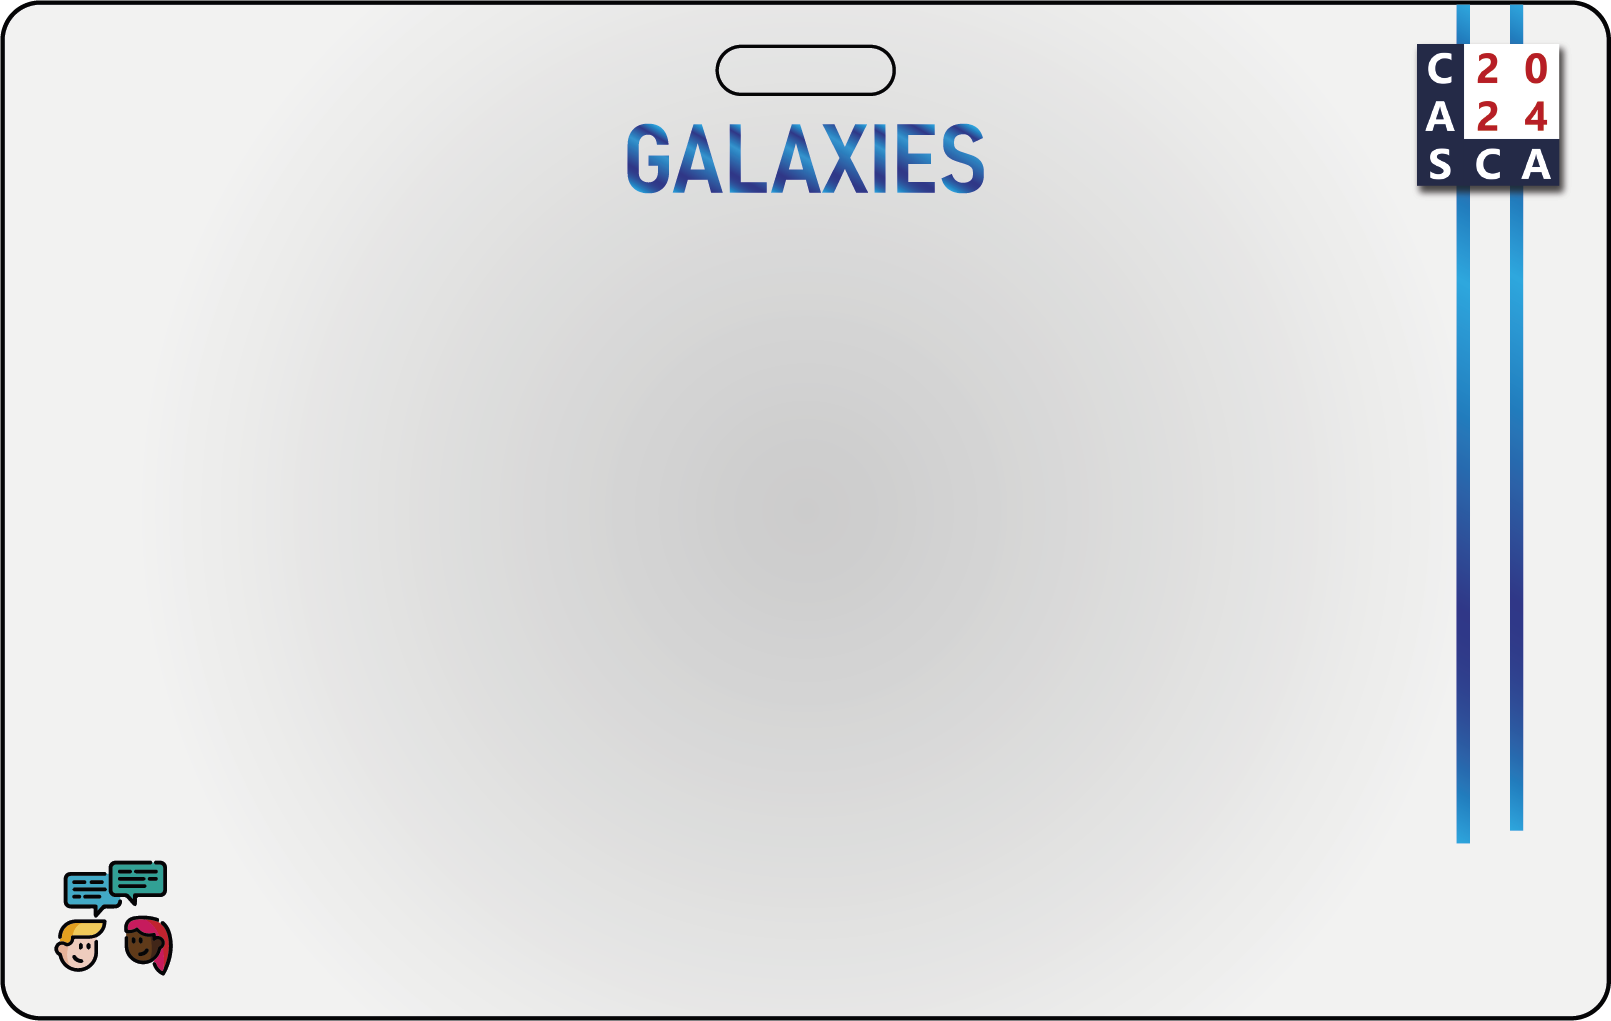
\includegraphics{Templates/Galaxies.png}}}
}

\participant{Lauren}{Foster}{McMaster University}{she/her}{English}{G}
% \renewcommand*{\ticketdefault}{%
\put(0,0){\lbox{
\includegraphics{Templates/ISM.png}}}
}

\participant{John}{Smith}{University of Calgary}{they/them}{English, French, Spanish, German}{U}
% \renewcommand*{\ticketdefault}{%
\put(0,0){\lbox{\includegraphics{Templates/Transients_Compact Objects.png}}}
}

\participant{Viraja}{Khatu}{Canada-France-Hawaii Telescope}{she/elle}{English}{P}
%%%%%%%%%%%%%%%%%%%%%%%%%%%%%%%%%%%
% end of the participant list
%%%%%%%%%%%%%%%%%%%%%%%%%%%%%%%%%%%
% empty tickets below
%\emptyticket{}
%\emptyticket{}
\end{document}
